\documentclass[11pt]{article}
\usepackage[margin=1in]{geometry}
\usepackage[T1]{fontenc}
\usepackage{lmodern}
\usepackage{microtype}
\usepackage{amsmath,amssymb}
\usepackage{booktabs,tabularx,array}
\usepackage{enumitem}
\usepackage{xcolor}
\usepackage{graphicx}
\usepackage{listings}
\usepackage[obeyspaces,spaces]{url}
\usepackage[hidelinks]{hyperref}

\setlist{itemsep=2pt,topsep=4pt}
\setlength{\parskip}{4pt}
\setlength{\emergencystretch}{3em}
\renewcommand{\arraystretch}{1.2}
\newcolumntype{Y}{>{\raggedright\arraybackslash}X}
\definecolor{notebg}{RGB}{238,244,252}
\definecolor{decbg}{RGB}{253,240,232}
\definecolor{codebg}{RGB}{247,247,250}
\definecolor{codeframe}{RGB}{200,200,210}
\lstset{basicstyle=\ttfamily\small, columns=fullflexible, keepspaces=true, backgroundcolor=\color{codebg},
  frame=single, rulecolor=\color{codeframe}, breaklines=true, xleftmargin=4pt, xrightmargin=4pt}
\newcommand{\code}[1]{\texttt{#1}}
\newcommand{\note}[1]{\par\noindent\colorbox{notebg}{\parbox{\dimexpr\linewidth-2\fboxsep}{\small\textbf{Note.} #1}}\par}
\newcommand{\decision}[1]{\par\noindent\colorbox{decbg}{\parbox{\dimexpr\linewidth-2\fboxsep}{\small\textbf{Decision needed.} #1}}\par}

\title{\textbf{Paratemporal Methods for Reinforcement Learning}\\[4pt]\large Plan and progress (RL track)}
\author{ParaDEVS Library workspace, Binghamton}
\date{Started October 10, 2026}

\newcommand{\docsdir}{../}
\def\thisdoc{rl}
% Shared cross-document links for the ParaDEVS documents. Each document defines \docsdir (path from its folder to
% docs/) and \thisdoc (its key below), then \input's this file.
%
% \doclink{path relative to docs/}{text}: a link to another PDF. Links are plain URI actions (file:///...), because
% Edge, Chrome and VS Code's PDF viewers ignore hyperref's usual "open another PDF" (GoToR) links. The absolute
% address comes from docroot.tex, which scripts/build_docs.sh regenerates; rerun it if the folder moves.
%
% \relateddocs: the "ParaDEVS documents" box listing every document, with the current one marked.
\InputIfFileExists{\docsdir docroot.tex}{}{\gdef\docroot{.}}
\providecommand{\thisdoc}{}
\definecolor{pdlink}{RGB}{20,80,170}
\definecolor{pdrelbg}{RGB}{243,246,252}
\definecolor{pdrelframe}{RGB}{190,200,220}
\makeatletter
\newcommand{\doclink}[2]{\hyper@linkurl{\textcolor{pdlink}{\textbf{#2}}}{\docroot/#1}}
\newcommand{\pd@item}[4]{% key, path, title, description
  \def\pd@key{#1}%
  \item \ifx\pd@key\thisdoc\textbf{#3} (this document)\else\doclink{#2}{#3}\fi: #4}
\newcommand{\relateddocs}{\par\medskip\noindent
  \fcolorbox{pdrelframe}{pdrelbg}{\parbox{\dimexpr\linewidth-2\fboxsep-2\fboxrule}{\small
  \textbf{ParaDEVS documents.} The entry point is \doclink{ParaDEVS_Start_Here.pdf}{Start Here}, a reading guide
  that links every document.
  \begin{itemize}[leftmargin=1.4em,itemsep=0pt,topsep=2pt]
  \pd@item{report}{report/ParaDEVS_Build_Report.pdf}{Build Report}{what has been built, how it was verified, what is next}
  \pd@item{howto}{howto/ParaDEVS_HowTo.pdf}{How-To Guide}{setup, tutorials, API reference, troubleshooting}
  \pd@item{architecture}{architecture/ParaDEVS_Architecture.pdf}{Architecture Guide}{how the library works and how to read results}
  \pd@item{rl}{rl/ParaDEVS_RL_Plan.pdf}{RL Plan}{reinforcement-learning plan, analysis and results}
  \pd@item{control}{rl/ParaDEVS_Control_Spec.pdf}{Control Spec}{action selection: Para.decide, graph-mode planning, value and policy iteration}
  \pd@item{hybrid}{rl/ParaDEVS_Hybrid_Study.pdf}{Hybrid Study}{which draws to enumerate or sample, and how cost grows with lookahead}
  \pd@item{fastcopy}{engine/ParaDEVS_FastCopy_Proposal.pdf}{Fast-Copy Proposal}{why the engine replays steps, where time goes, how to speed it up}
  \end{itemize}}}\par\medskip}
\makeatother


\begin{document}
\maketitle

\begin{abstract}
\noindent This plan identifies where the paratemporal engine (exact or sampled branching with merging) can give
reinforcement learning something standard methods do not. It analyses the variance consequences of Monte Carlo
sampling at every stage combined with merging, proposes toy problems with known answers and standard Python baselines,
and surveys how the Java/MS4 engine and a Python learner should communicate. A progress section records what has been
built (Section~\ref{sec:progress}).
\end{abstract}

\relateddocs

\tableofcontents

%=====================================================================
\section{Where we are today}
\begin{itemize}
\item The Demo Deliverable's RL side is \path{ParaDEVS_Barb_Q_Constructor.ipynb} (Colab, PyTorch). It runs tabular
  Q-learning on stock CSVs, then \textbf{row-normalises the Q-table into action probabilities} and saves it as a CSV.
  The Java engine reads that CSV as a stochastic policy (the \code{Trader} model in the finance port).
\item So today the engine does \textbf{policy evaluation}: the exact distribution of returns of a fixed stochastic
  policy in a stochastic environment. The integration is offline, through a file. The Demo README's
  \code{ms4me.para(env, action, state, N)} is the intended online interface and does not exist yet.
\item Library v0 supports a fixed input trace only. An agent that reacts to outputs (``reactive inputs'') is future work.
\end{itemize}

%=====================================================================
\section{Where paratemporal fits in RL}
\begin{center}
\small
\begin{tabularx}{\linewidth}{@{}p{2.6cm} Y Y Y@{}}
\toprule
\textbf{Use} & \textbf{Engine provides} & \textbf{Standard alternative} & \textbf{Why it might win}\\
\midrule
A. Policy evaluation & exact $V^\pi(s)$ and the full return distribution & many Monte Carlo rollouts; TD & no sampling variance where draws are discrete and merge well\\
B. n-step targets & $E[G_{t:t+n}]$ from $s_t$, exact or sampled with merging, leaves bootstrapped from the learner's $V$ & one sampled n-step return; tree backup; $Q(\sigma)$ & lower-variance targets; generalises Expected SARSA and tree backup to stochastic environments with a simulator\\
C. Distributional targets & the distribution of the n-step return & C51, QR-DQN learn it by sampling & exact target distributions; risk measures such as CVaR for finance\\
D. Lookahead for control & sparse sampling or tree search over the DEVS model, merging turns the tree into a DAG & MCTS, sparse sampling (Kearns, Mansour \& Ng 2002) & merging handles transpositions; exactness on small branches\\
\bottomrule
\end{tabularx}
\end{center}
\textbf{Recommended first target: B (n-step targets), with A as its special case} ($n\to$ episode end). It is closest
to the proposed method, has a clean ground truth, and plugs into any TD learner.

%=====================================================================
\section{Monte Carlo at every stage, plus merging: variance}
\label{sec:variance}

\paragraph{Setup.} At each stage every live node draws $k$ children of weight $w/k$. After the stage, nodes in the same
state are merged and their weights added. The concern: merging means fewer sample paths are drawn than without merging.

\paragraph{Theory.}
\begin{itemize}
\item \textbf{Unbiased either way.} A child carries $w/k$, so $E[\sum_i (w/k) f(v_i)] = w\,E f$. Merging equal
  continuations and sampling their future afresh preserves this (main\_paratemporal, Proposition ``Safe merging'',
  sampled case).
\item \textbf{Why variance rises with a fixed $k$.} Two nodes of weights $w_1, w_2$ in the same state, $\sigma^2$ the
  variance of one sampled estimate of that state's future. Unmerged, they have independent futures:
  $(w_1^2+w_2^2)\sigma^2/k$. Merged, they share one: $(w_1+w_2)^2\sigma^2/k$, larger by $2w_1w_2\sigma^2/k$. Merging
  with a fixed $k$ discards independent samples, as suspected, and also saves the work of drawing them.
\item \textbf{The fix is reallocation.} Keep a per-stage budget $B$ and give merged node $i$ $n_i\approx B\,w_i/W$ children
  (at least one), each of weight $w_i/n_i$. Unbiasedness holds because $n_i$ depends only on the past. Since the choice
  depends on weights, it falls outside the paper's merge proposition and needs its own short argument; dropping nodes
  ($n_i=0$) requires Russian roulette to stay unbiased.
\item \textbf{Safe merging rarely fires in RL.} It requires equal observations, so accumulated returns must match too;
  with continuous rewards they almost never do. Merging on state only while carrying the probability-weighted
  accumulated return $A=\sum w\,G_{\text{past}}$ is exact for \emph{expectations}, by linearity
  ($E[G]=\sum_s A_s+\sum_s W_s\,E[G_{\text{future}}\mid s]$), but loses the return \emph{distribution}. This is the old IH
  idea with a precise validity condition: a linear objective and an additive reward.
\end{itemize}

\paragraph{Experiment} (\path{rl/experiments/merge_variance.py}). 19-state random walk, start 13, 6-step target
bootstrapped with $V(s)=(s-10)/10$, step reward $s'/100$ so that returns differ between paths, 1000 replications.
Work counts transitions sampled.
\begin{center}
\small
\begin{tabular}{@{}lrrrr@{}}
\toprule
\textbf{Estimator} & \textbf{Mean} (exact 1.08) & \textbf{Variance} & \textbf{Work} & \textbf{Var $\times$ work}\\
\midrule
exhaustive + accumulator merge & \textbf{1.08000 exact} & 0 & \textbf{42} & 0\\
tree, $k=3$, no merge & 1.0796 & 1.16e-2 & 1092 & 12.7\\
tree, $k=3$, safe merge & 1.0788 & 1.95e-2 & 106 & 2.07\\
tree, $k=3$, accumulator merge & 1.0827 & 2.40e-2 & 51 & 1.23\\
budget $B=9$/stage & 1.0775 & 1.23e-2 & 54 & 0.66\\
budget $B=182$/stage (= tree work) & 1.0799 & \textbf{6.6e-4} & 1092 & 0.72\\
plain MC, $N=9$ rollouts & 1.0786 & 1.29e-2 & 54 & 0.70\\
plain MC, $N=182$ rollouts & 1.0812 & 5.8e-4 & 1092 & 0.63\\
\bottomrule
\end{tabular}
\end{center}
All estimators are unbiased (each mean within 1.6 standard errors of 1.08).

\paragraph{What this means.}
\begin{enumerate}
\item A fixed-$k$ tree without merging is the worst use of samples: its $k^n$ leaves share ancestors.
\item Merging with a fixed $k$ is about $20\times$ cheaper and about $2\times$ noisier, a net $6$--$10\times$ gain.
\item Merging with budget reallocation, at the work of the unmerged tree, gives $17\times$ lower variance and ties with
  plain independent rollouts per unit of work.
\item With sampling everywhere, merging cannot beat plain Monte Carlo. The engine's advantage is \textbf{exhaustive
  expansion with merging wherever outcome sets are small}. The design for n-step methods is therefore \textbf{hybrid}:
  enumerate small discrete draws, merge, and sample only large or continuous draws with budget reallocation.
\end{enumerate}
Open questions: allocation by weight or by weight $\times$ spread (Neyman allocation); effective sample size per stage;
repeating the study with larger branching and continuous noise.

%=====================================================================
\section{Toy problems}
\begin{center}
\small
\begin{tabularx}{\linewidth}{@{}p{0.7cm} p{4.0cm} Y p{2.8cm}@{}}
\toprule
\textbf{\#} & \textbf{Problem} & \textbf{Why} & \textbf{Ground truth}\\
\midrule
T1 & 19-state random walk (S\&B \S7.1) & the standard n-step TD benchmark (S\&B Fig.~7.2) & $V(s)=(s-10)/10$\\
T2 & FrozenLake 4$\times$4 / 8$\times$8, slippery (Gymnasium) & stochastic transitions, small state space so merging is very effective; control & value iteration\\
T3 & Blackjack (Gymnasium) & classic Monte Carlo control, discrete rewards (safe merging works) & known optimal policy\\
T4 & Admission control / $(s,S)$ inventory with random event times (DEVS-native) & real event times, semi-MDP: where DEVS beats step-based gyms & DP on the embedded chain\\
T5 & Finance single stock (existing port) & ties back to the Demo Deliverable; risk measures & engine exhaustive results\\
\bottomrule
\end{tabularx}
\end{center}
Order: T1 $\to$ T2 $\to$ T5 $\to$ T4; T3 optional.

%=====================================================================
\section{Python baselines}
\begin{center}
\small
\begin{tabularx}{\linewidth}{@{}p{4.4cm} Y@{}}
\toprule
\textbf{Framework} & \textbf{Use}\\
\midrule
Gymnasium (Farama) & environment API; FrozenLake, Blackjack, CliffWalking built in; our DEVS environments get a Gymnasium wrapper\\
Own tabular reference code & n-step TD, n-step SARSA, tree backup, $Q(\sigma)$ (S\&B ch.~7); transparent and the fairest baseline for T1/T2\\
Stable-Baselines3 + sb3-contrib & PPO, DQN, A2C; QR-DQN for distributional comparison\\
CleanRL & single-file implementations; easiest place to swap in engine-computed n-step targets\\
optional: MCTS baseline & own UCT, or DeepMind's JAX-based \code{mctx}, for use D\\
not now: RLlib, TorchRL, Tianshou & heavier; revisit if scale demands it\\
\bottomrule
\end{tabularx}
\end{center}

%=====================================================================
\section{Connecting the Java/MS4 engine to Python}

\paragraph{Two directions} (\path{Paper/DEVS-RL/DEVS-RL_Integration.png}).
\emph{DEVS into RL}: the DEVS model is the environment and a Python agent calls \code{reset}/\code{step}; the engine
must pause at a decision point and wait for an action, or for the policy's action probabilities to branch over.
\emph{RL into DEVS}: the agent is a DEVS component (like \code{Trader}) whose policy is a table or, later, an exported
network (ONNX inside Java). The second works today for tabular policies.

\paragraph{A unifying library feature: decision points.} Add \code{Para.decide(label, options)}, analogous to
\code{Para.choose}, whose law comes from a \emph{policy supplied at run time} (a table, or a callback into Python). The
engine treats it like any draw (exhaustive, sampled or hybrid), so one mechanism covers policy evaluation, n-step
targets and branching over actions. A Gymnasium \code{step(action)} is the special case of a policy that forces one
action.

\paragraph{Transport options.}
\begin{center}
\small
\begin{tabularx}{\linewidth}{@{}p{3.6cm} Y Y@{}}
\toprule
\textbf{Option} & \textbf{How} & \textbf{Fit}\\
\midrule
1. Files (today) & policy CSV $\to$ Java $\to$ results & offline tabular evaluation only\\
\textbf{2. JPype} (in-process) & the JVM runs inside Python (JNI); Python calls \code{ParaEngine} directly and can implement Java interfaces & \textbf{recommended first}: lowest latency, no server; verified working (Section~\ref{sec:progress})\\
2b. Py4J & a separate JVM reached over a local socket & simpler isolation, more overhead per call\\
3. Service & Java engine behind gRPC, REST or ZeroMQ & learners and simulators on different machines\\
4. Message broker & MQTT, Kafka or RabbitMQ between DEVS federates and agents & distributed, real-time or multi-framework co-simulation\\
\bottomrule
\end{tabularx}
\end{center}
Recommendation: one small Python API (\code{ParaEnv} for Gymnasium plus \code{para\_eval(state, policy, n, rule)}),
implemented first over JPype and kept independent of the transport.

\paragraph{The ``online DEVS message broker''.}
\begin{itemize}
\item \textbf{MS4 Me's built-in collaboration service is not a broker.} Inspected locally in the MS4 Me 1.5 plugins: a
  SOAP client for login, licences and the MS4 model store (upload, download and lock model jars).
\item \textbf{Closest match:} Dominici, Capocchi, Santucci, Koertje, Kewley, \emph{Broker-Based Distributed DEVS
  Simulation: Enabling Multi-Framework Interoperability through Message Broker Architecture}, SIMULTECH 2026,
  doi:10.5220/0014846100004094. Capocchi and Santucci created DEVSimPy (Python DEVS), so this is likely the
  Python-connectable broker remembered. Its broker technology and code availability could not be confirmed online.
  \textbf{To do: obtain the paper.}
\item Related: xDEVS (Java, Python, C++; distributed over sockets and, in 2025 work, MQTT); DEVS/SOA (web services).
\item Assessment: a broker matters for real-time or multi-framework co-simulation over a network. For RL training,
  where the learner calls the engine very often, an in-process bridge is the better first step.
\end{itemize}

%=====================================================================
\section{Phased plan}
\begin{center}
\small
\begin{tabularx}{\linewidth}{@{}p{2.3cm} Y p{4.2cm}@{}}
\toprule
\textbf{Phase} & \textbf{Work} & \textbf{Done when}\\
\midrule
R0 setup & project virtual environment; pinned gymnasium, stable-baselines3, jpype1; notebook run headless & notebook Q-table reproduced locally\\
R1 Python prototypes & reference estimators; n-step TD on T1 with single-path, exact, sampled+merge+budget and rollout targets; then T2 & learning curves showing where model-based targets win per unit of work\\
R2 library features & $k$-sample Monte Carlo rule; per-stage budget; accumulator merge (\emph{needs approval}); leaf-value hook; \code{Para.decide} & new Java acceptance tests pass\\
R3 bridge & JPype \code{ParaEnv} and \code{para\_eval}; T2 through the Java engine & Java matches the Python prototype\\
R4 baselines & T2/T5 (then T4) vs tabular code and SB3 & comparison report\\
R5 architecture & read Dominici et al.; decide on a service or broker & decision recorded\\
\bottomrule
\end{tabularx}
\end{center}

\decision{(1) Accumulator (expectation-only) merging as an opt-in in the Java library. Used in the Python prototypes
for now, not added to the library. (2) JPype-first integration: being followed, since it is the recommendation.
(3) Toy-problem order T1 $\to$ T2 $\to$ T5 $\to$ T4: being followed.}

%=====================================================================
\section{Progress}
\label{sec:progress}

\subsection{R0: environment (done 2026-10-10)}
\begin{itemize}
\item Virtual environment \path{rl/.venv} (Python 3.13, system site-packages for numpy). Pinned in
  \path{rl/requirements.txt}: gymnasium 1.4.0, stable-baselines3 2.9.0, sb3-contrib 2.9.0, jpype1 1.7.1, torch 2.14.1
  (inside the venv; the system torch 2.7 is untouched), matplotlib 3.11.2, pandas 2.3.3, numpy 2.3.4.
\item \textbf{JPype bridge verified}: \path{rl/scratch/jpype_smoke.py} starts the JVM from Python, implements the Java
  \code{Transducer} and \code{Supplier} interfaces in Python, runs the tutorial \code{ServiceLine} through the Java
  \code{ParaEngine}, and gets the exact result ($P(3\text{ served})=0.36$, $P(2)=0.64$).
\item \textbf{Q-table notebook runs headless}: \path{rl/baselines/q_table_constructor.py} ports the notebook's
  training cells (numpy instead of torch, a seed, no Colab). Trained on \path{Train_AAPL.csv} with 15 shares it reproduces
  the Demo's \path{Q_table_AAPL_stoch_1_15.csv} to within about 1\% per entry (buy probability in row 0: 0.792 vs 0.795;
  the difference is the random seed). Runs in about 7 s.
\end{itemize}

\note{\textbf{Finding about the existing RL reward.} The notebook's reward is 1 when the new holding equals the
reachable holding of largest value $\sum \text{shares}\times\text{price}$ at the current date. With positive prices that
is always the largest share count, so the reward means ``buy'' (or hold at the cap), regardless of price movements. The
learned policies are therefore buy-biased by construction (about 80\% buy in every row) and carry no information about
price dynamics. For T5 the reward should be redesigned, for example as the change in portfolio value, before policies
from it are interpreted as trading strategies.}

\subsection{R1: Python reference prototypes (in progress)}
\path{rl/paratemporal_py} implements tabular Markov reward processes and four n-step target estimators: exact
(exhaustive expansion with merging), budgeted sampling with merging, independent rollouts, and the classic trajectory
return. Under expectation merging the merged nodes at a stage form a weight vector over states, so the estimators are
vectorised. \path{rl/tests/test_targets.py} checks Bellman consistency (with the true $V$, every exact n-step target
equals $V(s)$, to $10^{-12}$), agreement with matrix powers, and unbiasedness of the sampled estimators. All pass.
\path{paratemporal_py.frozen_lake} loads the exact slippery-FrozenLake model from Gymnasium; its exact 100-step success
probability under the optimal policy (0.7402) matches Gymnasium's own Monte Carlo ($0.741\pm0.003$).

Done: prediction studies on T1 and T2 (below). Remaining in R1: T2 control, hybrid selection, and the
work-saturation study.

% Results of R1 experiments. Tables and figures are generated by rl/experiments/make_tex_tables.py from the JSON
% results; the interpretation below is written by hand.

\paragraph{Setup.} Each study compares four ways of forming the target for updating $V(S_t)$. (A) Classic n-step TD
uses only the agent's own trajectory (model-free). (B) The exact expected n-step target is computed by exhaustive
expansion with merging. (C) The sampled target uses merging and a per-stage budget of 4. (D) The target averages
4 independent rollouts. B, C and D query a simulator from every visited state, which is the paratemporal setting.
Two costs therefore matter separately: \emph{real experience} (episodes) and \emph{compute} (work, the transitions
examined or sampled). Both runs were restarted in the foreground with incremental saving after an out-of-memory kill.

\subsection{T1: 19-state random walk, n-step TD prediction}
\label{sec:t1}
\begin{center}\small
\begin{tabular}{@{}lrrrr@{}}
\toprule
\textbf{Target} & \textbf{n=1} & \textbf{n=2} & \textbf{n=4} & \textbf{n=8}\\
\midrule
A: n-step TD (model-free) & 0.345\,$\pm$\,0.002 & 0.276\,$\pm$\,0.004 & 0.263\,$\pm$\,0.005 & 0.277\,$\pm$\,0.005\\
\quad best $\alpha$, work/episode & $\alpha$=0.8, 99 & $\alpha$=0.6, 99 & $\alpha$=0.4, 99 & $\alpha$=0.2, 99\\[2pt]
B: exact (exhaustive + merge) & 0.285\,$\pm$\,0.005 & 0.238\,$\pm$\,0.006 & 0.181\,$\pm$\,0.006 & 0.139\,$\pm$\,0.006\\
\quad best $\alpha$, work/episode & $\alpha$=1, 296 & $\alpha$=1, 687 & $\alpha$=1, 2{,}030 & $\alpha$=1, 6{,}693\\[2pt]
C: sampled + merge + budget & 0.305\,$\pm$\,0.006 & 0.279\,$\pm$\,0.005 & 0.239\,$\pm$\,0.005 & 0.217\,$\pm$\,0.004\\
\quad best $\alpha$, work/episode & $\alpha$=1, 495 & $\alpha$=1, 886 & $\alpha$=0.8, 1{,}711 & $\alpha$=0.6, 3{,}268\\[2pt]
D: independent rollouts & 0.305\,$\pm$\,0.006 & 0.280\,$\pm$\,0.005 & 0.242\,$\pm$\,0.005 & 0.218\,$\pm$\,0.005\\
\quad best $\alpha$, work/episode & $\alpha$=1, 495 & $\alpha$=1, 913 & $\alpha$=0.8, 1{,}632 & $\alpha$=0.6, 3{,}231\\[2pt]
\bottomrule
\end{tabular}
\end{center}
\noindent Best step size per cell. RMS error over the 19 states, averaged over the first 10 episodes and 100 runs. Work counts transitions examined or sampled, including the agent's own steps.

\begin{figure}[h]\centering
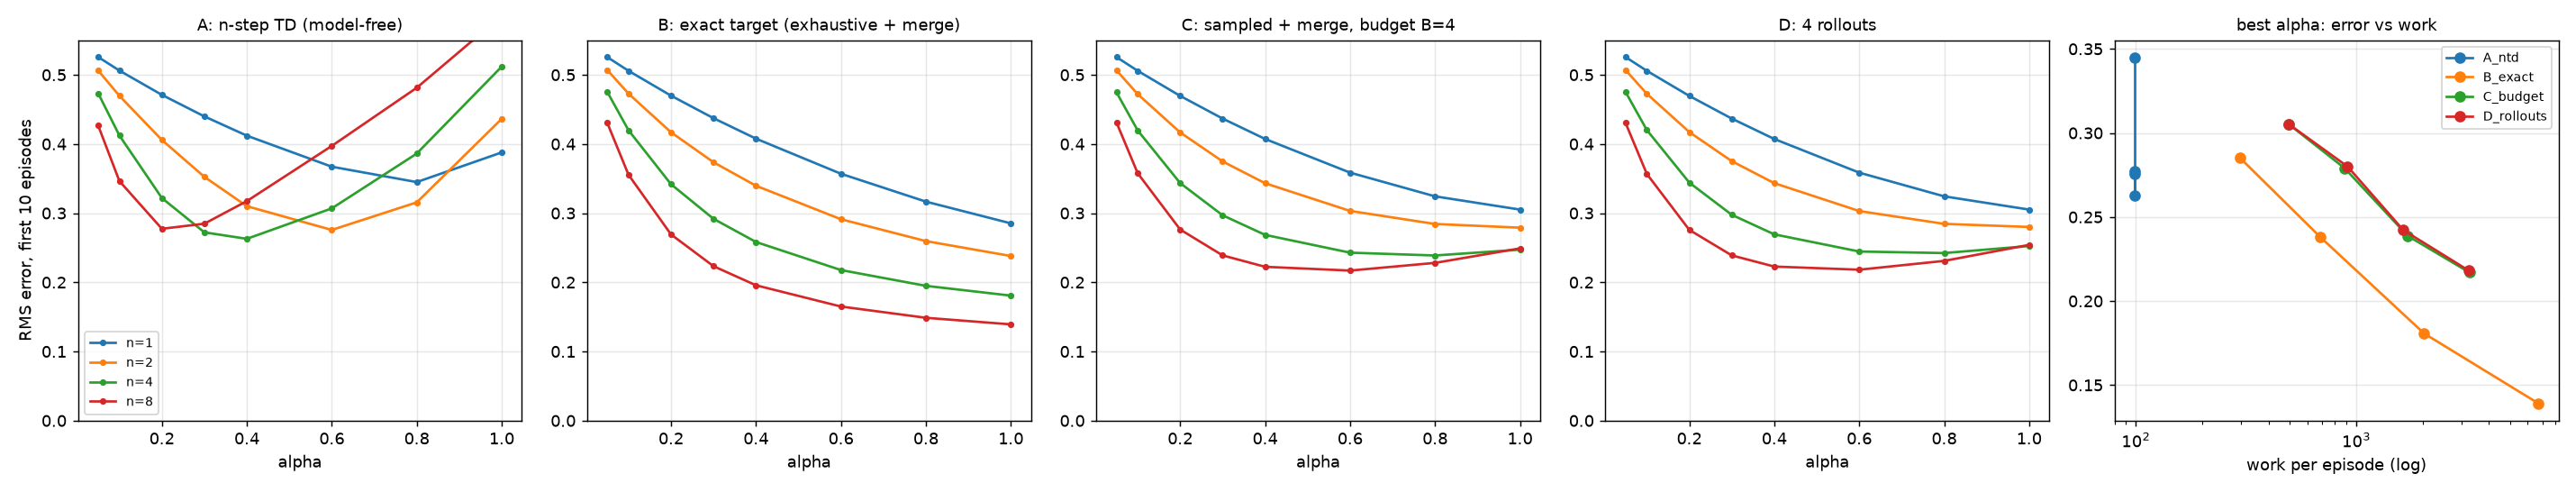
\includegraphics[width=\linewidth]{t1_nstep_td.png}
\caption{T1: 19-state random walk, n-step TD prediction: error against step size for each target, and best-$\alpha$ error against work.}
\end{figure}



\subsection{T2: slippery FrozenLake 8$\times$8, prediction}
\label{sec:t2}
\begin{center}\small
\begin{tabular}{@{}lrrrr@{}}
\toprule
\textbf{Target} & \textbf{n=1} & \textbf{n=2} & \textbf{n=4} & \textbf{n=8}\\
\midrule
A: n-step TD (model-free) & 0.185\,$\pm$\,0.002 & 0.174\,$\pm$\,0.002 & 0.166\,$\pm$\,0.002 & 0.161\,$\pm$\,0.002\\
\quad best $\alpha$, work/episode & $\alpha$=0.6, 42 & $\alpha$=0.4, 42 & $\alpha$=0.4, 42 & $\alpha$=0.2, 42\\[2pt]
B: exact (exhaustive + merge) & 0.159\,$\pm$\,0.002 & 0.137\,$\pm$\,0.002 & 0.114\,$\pm$\,0.003 & 0.094\,$\pm$\,0.003\\
\quad best $\alpha$, work/episode & $\alpha$=1, 205 & $\alpha$=1, 804 & $\alpha$=1, 4{,}067 & $\alpha$=1, 21{,}502\\[2pt]
C: sampled + merge + budget & 0.168\,$\pm$\,0.002 & 0.147\,$\pm$\,0.003 & 0.135\,$\pm$\,0.003 & 0.124\,$\pm$\,0.002\\
\quad best $\alpha$, work/episode & $\alpha$=1, 201 & $\alpha$=1, 380 & $\alpha$=0.8, 676 & $\alpha$=0.6, 1{,}358\\[2pt]
D: independent rollouts & 0.168\,$\pm$\,0.002 & 0.150\,$\pm$\,0.003 & 0.135\,$\pm$\,0.003 & 0.123\,$\pm$\,0.002\\
\quad best $\alpha$, work/episode & $\alpha$=1, 201 & $\alpha$=1, 359 & $\alpha$=0.8, 694 & $\alpha$=0.6, 1{,}227\\[2pt]
\bottomrule
\end{tabular}
\end{center}
\noindent Best step size per cell. RMS error over nonterminal states, averaged over the first 30 episodes and 50 runs (exploring starts; $\varepsilon=0.2$-soft optimal policy; $\gamma=0.99$). Work counts transitions examined or sampled, including the agent's own steps.

\begin{figure}[h]\centering
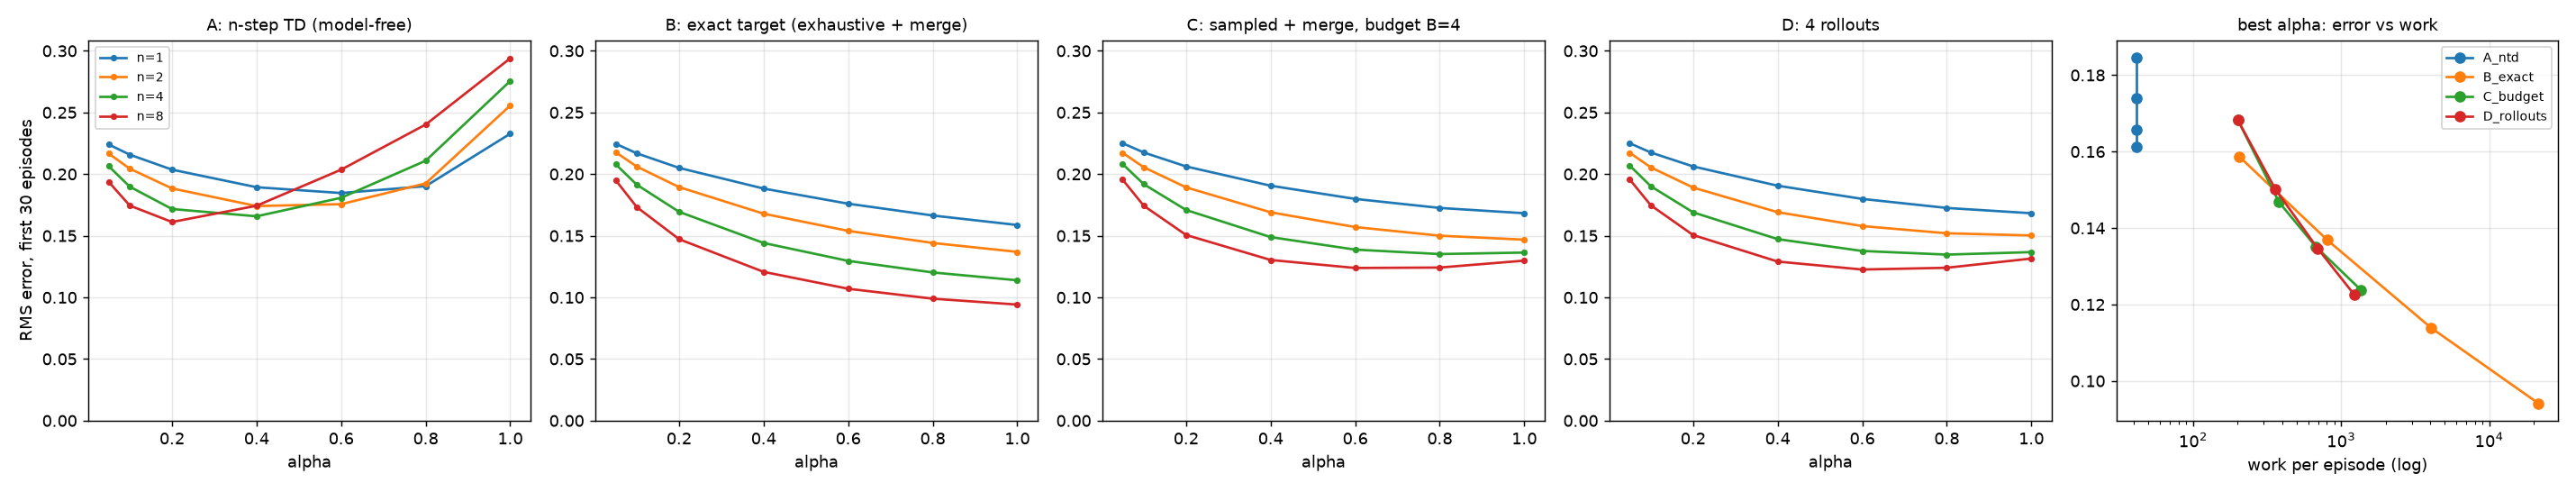
\includegraphics[width=\linewidth]{t2_frozenlake_prediction.png}
\caption{T2: slippery FrozenLake 8$\times$8, prediction: error against step size for each target, and best-$\alpha$ error against work.}
\end{figure}



\subsection{What R1 shows}
\begin{enumerate}
\item \textbf{The baseline is reproduced.} A reproduces Sutton \& Barto's Figure 7.2 on T1: intermediate n is best
  ($n=4$, RMS 0.263 at $\alpha=0.4$), with the characteristic U-shaped curves in $\alpha$.
\item \textbf{Per episode of real experience, the exact target wins clearly.} On T1, B with $n=8$ reaches RMS
  $0.139$ against $0.263$ for the best model-free setting, roughly half the error after the same 10 episodes. On T2 it is
  $0.094$ against $0.161$. B's error falls steadily with $n$ and is best at $\alpha=1$ in every cell: the exact target
  has no sampling noise, so there is no reason to average it.
\item \textbf{Merging with a budget ties with independent rollouts, again.} C and D agree within one standard error in
  every cell of both studies (e.g. T1, $n=8$: $0.217$ vs $0.218$; T2, $n=8$: $0.124$ vs $0.123$). This matches the
  variance study in Section~\ref{sec:variance}: for sampled expected-value targets, merging with reallocation is as
  good as, but not better than, independent sampling.
\item \textbf{Per unit of compute, the picture depends on the problem.} On T1 the exact target dominates the sampled ones
  at equal work (right panel: B's curve lies below C and D everywhere; e.g. $0.181$ at 2{,}030 work vs $0.217$ at about
  3{,}250). On T2 the three are about level at equal work (e.g. B $n=2$: $0.137$ at 804; C/D $n=4$: $0.135$ at about
  690). B buys lower error at higher cost, because an $\varepsilon$-soft policy on slippery ice has up to 12 successors per
  state and the merged frontier quickly covers much of the grid.
\item \textbf{Against model-free TD, the comparison is about which resource is scarce.} B--D spend 3--500$\times$ more work
  per episode than A. If real experience is expensive and a simulator is available (the DEVS setting), the paratemporal
  targets are much better. If compute and experience cost the same, model-free TD with more episodes remains
  competitive on these small problems.
\end{enumerate}

\paragraph{Consequences for the next phases.}
\begin{itemize}
\item The case for exact expansion with merging is strongest when the \emph{reachable merged frontier stays small}:
  work per target is bounded by $n \times |\text{frontier}| \times \text{branching}$, independent of the number of paths,
  while a sampled estimate needs ever more samples for the same accuracy. Next: measure where exact expansion's work
  saturates as $n$ grows, and how many samples C/D need to match B's error.
\item Hybrid selection (exact on small discrete draws, sampled elsewhere) is the configuration to test next. On T2 the
  natural split is to enumerate the slip (3 outcomes) and sample the policy, or the reverse.
\item Control (T2 with n-step Q-learning or SARSA targets) and the Java engine via JPype (R3) are the next steps. The
  Python estimators above are the reference the Java results must match.
\end{itemize}


\end{document}
